\documentclass[a4paper]{article}
\usepackage{amsmath,amssymb,caption,float,geometry,graphicx,xcolor}
\captionsetup[figure]{labelsep=period}
\geometry{left=3.5cm,right=3.5cm,top=3.3cm,bottom=3.3cm}
\renewcommand\thesection{\arabic{section}}
\begin{document}
\begin{center}
\huge
\textbf{VE320\\Intro to Semiconductor Devices\\}
\Large
\vspace{30pt}
\uppercase{Homework 8}\\
\vspace{5pt}\today\\
\vspace{5pt}
Yihua Liu 518021910998
\vspace{5pt}
\rule[-10pt]{.97\linewidth}{0.05em}
\end{center}
1. (a) (a) The semiconductor is p type.\\
(b) The semiconductor is p type.\\
(c) The semiconductor is p type.\\
(d) The semiconductor is n type.

(b) (a) The device is biased in the inversion region.\\
(b) The device is biased in the depletion region.\\
(c) The device is biased in the accumulation region.\\
(d) The device is biased in the strong inversion region.

(c) (a)
\begin{figure}[H]
    \centering
    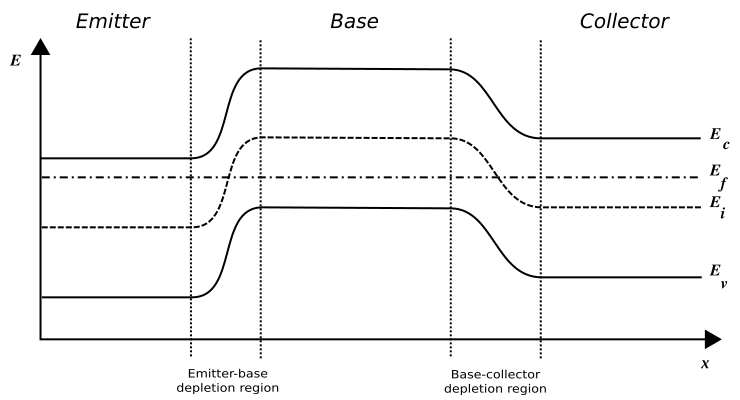
\includegraphics[width=1\textwidth]{1.png}
    \caption{1(c)(a).}
\end{figure}
(b)
\begin{figure}[H]
    \centering
    \includegraphics[width=1\textwidth]{2.png}
    \caption{1(c)(b).}
\end{figure}
(c)
\begin{figure}[H]
    \centering
    \includegraphics[width=1\textwidth]{3.png}
    \caption{1(c)(c).}
\end{figure}
(d)
\begin{figure}[H]
    \centering
    \includegraphics[width=1\textwidth]{4.png}
    \caption{1(c)(d).}
\end{figure}

2. (a) The ideal flat-band voltage is
\[V_{FB}=\phi_{ms}=-0.4\,\text{V}.\]

(b) (i) The shift in flat-band voltage is
\[\Delta V_{FB}=-\frac{Q_{ss}'}{C_\text{ox}}=-\frac{4\times10^{10}e}{\frac{3.9\times0.01\epsilon_0}{200\times10^{-8}}}=-0.0371\,\text{V}.\]
(ii) The shift in flat-band voltage is
\[\Delta V_{FB}=-\frac{Q_{ss}'}{C_\text{ox}}=-\frac{10^{11}e}{\frac{3.9\times0.01\epsilon_0}{200\times10^{-8}}}=-0.0928\,\text{V}.\]

(c) The ideal flat-band voltage is
\[V_{FB}=\phi_{ms}=-0.4\,\text{V}.\]
(i) The shift in flat-band voltage is
\[\Delta V_{FB}=-\frac{Q_{ss}'}{C_\text{ox}}=-\frac{4\times10^{10}e}{\frac{3.9\times0.01\epsilon_0}{120\times10^{-8}}}=-0.0223\,\text{V}.\]
(ii) The shift in flat-band voltage is
\[\Delta V_{FB}=-\frac{Q_{ss}'}{C_\text{ox}}=-\frac{10^{11}e}{\frac{3.9\times0.01\epsilon_0}{120\times10^{-8}}}=-0.0557\,\text{V}.\]

3. The threshold voltage is
\[V_{TN}=(|Q_{SD}'(\text{max})|-Q_{ss}')\left(\frac{t_\text{ox}}{\epsilon_\text{ox}}\right)+\phi_{ms}+2\phi_{fp}\]
\[|Q_{SD}'(\text{max})|=eN_ax_{dT}=\sqrt{4eN_a\epsilon_s\phi_{fp}}\]
The difference between $E_{Fi}$ and $E_F$ is
\[\phi_{fp}=V_t\ln{\left(\frac{N_a}{n_i}\right)}=\frac{kT}{e}\ln{\left(\frac{N_a}{n_i}\right)}\]
The metal-semiconductor work function difference is
\[\phi_{ms}=\phi_m'-\left(\chi'+\frac{E_g}{2e}+\phi_{fp}\right).\]
For an aluminium-silicon dioxide junction, $\phi_m'=3.20$ V and, for a silicon-silicon dioxide junction, $\chi'=3.25$ V. We may assume that $E_g=1.12$ V. Then, the metal-semiconductor work function difference is
\[\phi_{ms}=2.30-\left(3.25+\frac{1.12e}{2e}+\phi_{fp}\right)=-0.61-\phi_{fp}.\]
Thus, the threshold voltage is
\[V_{TN}=(\sqrt{4eN_a\epsilon_s\phi_{fp}}-Q_{ss}')\left(\frac{t_\text{ox}}{\epsilon_\text{ox}}\right)-0.61+\phi_{fp}=+0.45\,\text{V}.\]
Solving the equation, the p-type doping concentration is
\[N_a=4.870\times10^{16}\,\mathrm{cm^{-3}}.\]

4. (a) The flat-band voltage is
\[V_{FB}=\phi_{ms}-\frac{Q_{ss}'}{C_\text{ox}}=-1.1-\frac{6\times10^{10}e}{\frac{3.9\times0.01\epsilon_0}{180\times10^{-8}}}=-1.150\,\text{V}.\]

(b) The difference between $E_{Fi}$ and $E_F$ is
\[\phi_{fp}=\frac{kT}{e}\ln{\left(\frac{N_a}{n_i}\right)}=\frac{300k}{e}\ln{\left(\frac{10^{15}}{1.5\times10^{10}}\right)}=0.287\,\text{V}.\]
The threshold voltage is
\[
    \begin{aligned}
        V_{TN}&=(\sqrt{4eN_a\epsilon_s\phi_{fp}}-Q_{ss}')\left(\frac{t_\text{ox}}{\epsilon_\text{ox}}\right)+\phi_{ms}+2\phi_{fp}\\
        &=(\sqrt{4e\times10^{15}\times11.7\times0.01\epsilon_0\phi_{fp}}-6\times10^{10}e)\left(\frac{180\times10^{-8}}{3.9\times0.01\epsilon_0}\right)-1.1+2\phi_{fp}\\
        &=-0.504\,\text{V}.
    \end{aligned}
\]

5. (a) The semiconductor is n type.

(b) The capacitance per unit area is
\[C_\text{ox}=\frac{C}{A}=\frac{200\times10^{-12}}{2\times10^{-3}}=10^{-7}\,\mathrm{F/cm^2}.\]
The oxide thickness is
\[t_\text{ox}=\frac{\epsilon_\text{ox}}{C_\text{ox}}=\frac{3.9\times0.01\epsilon_0}{10^{-7}}=3.453\times10^{-6}\,\text{cm}.\]

(c) We have
\[V_{FB}=\phi_{ms}-\frac{Q_{ss}'}{C_\text{ox}}.\]
The equivalent trapped oxide charge density is
\[Q_{ss}'=(\phi_{ms}-V_{FB})C_\text{ox}=(-0.50+0.8)\times10^{-7}=3\times10^{-8}\,\mathrm{C/cm^2}.\]

(d) The flat-band capacitance is
\[
    \begin{aligned}
        C_{FB}'&=\frac{\epsilon_\text{ox}}{t_\text{ox}+\left(\dfrac{\epsilon_\text{ox}}{\epsilon_s}\right)\sqrt{\left(\dfrac{kT}{e}\right)\left(\dfrac{\epsilon_s}{eN_a}\right)}}\\
        &=\frac{3.9\times0.01\epsilon_0}{\dfrac{3.9\times0.01\epsilon_0}{10^{-7}}+\dfrac{3.9\times0.01\epsilon_0}{11.7\times0.01\epsilon_0}\sqrt{\left(\dfrac{300k}{e}\right)\left(\dfrac{11.7\times0.01\epsilon_0}{2\times10^{16}e}\right)}}\\
        &=7.818\times10^{-8}\,\mathrm{F/cm^2}.
    \end{aligned}
\]
\end{document}